\documentclass[conference]{IEEEtran}
\usepackage{amsmath,amssymb,booktabs,array,url,graphicx}
\graphicspath{{figures/}}
\usepackage{iftex}
\ifPDFTeX\else
\usepackage{fontspec}
\setmainfont{texgyretermes}[Extension=.otf,UprightFont=*-regular,BoldFont=*-bold,ItalicFont=*-italic,BoldItalicFont=*-bolditalic,NFSSFamily=ptm]
\fi
\usepackage{pgfplots}
\pgfplotsset{compat=1.18}
\definecolor{preactblue}{HTML}{246693}
\definecolor{preactorange}{HTML}{C65B32}
\definecolor{preactgreen}{HTML}{39866E}
\title{Cross-System Transfer in Prefix-Based Software-Agent Failure Prediction}
\author{\IEEEauthorblockN{Yuvaraj Nayak}\IEEEauthorblockA{Department of Computer Science\\BITS Pilani, Dubai Campus\\Dubai, United Arab Emirates\\f20230006@dubai.bits-pilani.ac.in}}
\begin{document}
\maketitle
\begin{abstract}
Prefix-based monitors may identify unsuccessful software-agent runs, but their reliability can depend on the agent system, task partition, and which trajectories reach the prediction checkpoint. We audit inexpensive structural monitors on 1,665 public trajectories from three systems attempting the same 111 repository tasks. On one task-grouped partition at 20 tool results, source-system AUROC is 0.700, unchanged transfer to Qwen yields 0.456, and target-specific training yields 0.691. However, the paired target-trained minus transferred AUROC difference is 0.235 with a task-bootstrap 95\% interval of $[-0.071,0.459]$. Three repeated five-fold grouped evaluations produce transfer AUROC 0.463--0.562 and target-trained AUROC 0.497--0.558 at that checkpoint; the advantage changes sign. Eligibility is strongly system- and outcome-dependent. Target-validation adaptation improves Brier from 0.300 to 0.229 without improving ranking or outperforming a constant target-validation prior (0.223). These sensitivity analyses qualify the original finding: one favorable partition does not establish target-training superiority or isolate a model-weight effect. We provide pinned provenance and complete multi-checkpoint results. This observational study measures no prevention or intervention benefit.
\end{abstract}
\begin{IEEEkeywords}
software agents, failure prediction, cross-system transfer, grouped evaluation, calibration
\end{IEEEkeywords}

\section{Introduction}
Tool-using language-model agents interleave reasoning, actions and observations~\cite{react}. Long unsuccessful runs can expend considerable execution resources, motivating early outcome monitoring. Reflection~\cite{reflexion}, process feedback~\cite{sweprm}, and recovery architectures~\cite{selfhealing} address related reliability problems. Nevertheless, predicting eventual failure is distinct from preventing it: an accurate critic can disrupt runs that would succeed~\cite{interventionparadox}.

Early prediction, transfer, calibration and executed repair already have substantial precedents. The relevant empirical question here is narrower: \emph{how stable are inexpensive structural outcome predictors across task partitions, checkpoint populations, and a change of agent system?} We use ``system'' because the public traces vary model and scaffold jointly. We do not identify a model-only effect or present a completed predictive intervention controller.

The PreAct analysis package initially showed a sizable single-partition transfer contrast. We extend that pilot with paired task-cluster inference, repeated grouped evaluation, outcome-stratified checkpoint eligibility, common-cohort sensitivities, prior adjustment, target-validation calibration and feature-shift diagnostics. These additional sensitivity analyses evaluate the stability of the initial finding. All four checkpoints are reported; the emphasis on 20 results was chosen after the original test results and is not a preregistered primary endpoint. Our primary contribution is an evaluation protocol that exposes how a promising single-split cross-system prediction result becomes inconclusive under paired inference, repeated task-grouped evaluation, and eligibility/calibration checks. This is a reliability audit of structural monitors.

\section{Related Work and Positioning}
PrefixGuard learns event sequences for horizon-specific risk~\cite{prefixguard}; weak supervision addresses sparse early evidence~\cite{sparse}. AgentForesight audits decisive-error prefixes~\cite{agentforesight}, ProMAS forecasts semantic transitions~\cite{promas}, and trajectory graphs supply pre-execution diagnostics~\cite{graphcopilot}. Early termination and model switching also precede this study~\cite{agentstop,atropos}. Table~\ref{tab:position} contrasts the closest settings. Their different targets and budgets prevent direct numerical ranking against our monitor.

FailFast--RestartSmart uses a 0.6B prefix monitor on SWE-bench Verified, transfers from Qwen to other policies, and executes artifact-preserving restart~\cite{failfast}. EarlyEval uses LightGBM behavior/text/reference-solution features across three benchmarks, with leave-one-agent-out prediction for cheaper evaluation~\cite{earlyeval}. Dubey studies telemetry detection, serving-specific transfer/recalibration, and matched-checkpoint repair~\cite{sentinel}. We instead audit 20 structural features on a separate 111-task SWE-Rebench cohort, use task-grouped repeated evaluation, and separate ranking, probability adaptation and checkpoint selection. We do not claim that transfer failure or recalibration was first discovered here.

Outcome labels also have limits: AgentLens finds defects in passing runs~\cite{agentlens}; evaluator disagreements appear in AgentRewardBench~\cite{agentrewardbench}; early error onset need not coincide with visible evidence~\cite{failureprocess}. Cao's target-specific calibration audit is another predecessor~\cite{calibrationaudit}. ProbGuard and AgentSpec respectively predict unsafe reachability and enforce runtime rules~\cite{probguard,agentspec}. Executed debugging interventions in DoVer differ from imagined counterfactual corrections in A2P~\cite{dover,a2p}. The inspected self-healing paper says its experiments are ongoing; we treat it as a proposal~\cite{selfhealing}. The supplementary 40-paper evidence map retains source locations and qualified classifications; it is a targeted extraction, not independently double-screened synthesis.

\begin{table*}[t]
\centering\footnotesize
\caption{Closest-study comparison. Prior-study findings are author-reported, not reproduced by our experiments.}
\label{tab:position}
\begin{tabular}{@{}p{.18\textwidth}p{.26\textwidth}p{.27\textwidth}p{.22\textwidth}@{}}
\toprule Study & Data / representation & Evaluation purpose & Distinction from this audit \\
\midrule
FailFast~\cite{failfast} & SWE-bench Verified; learned 0.6B prefix monitor & Cross-policy warning and executed restart & Different dataset; task/budget success and resource effects \\
EarlyEval~\cite{earlyeval} & Three benchmarks; behavior, text, reference features & Held-out-agent verdict prediction and halting & Benchmark-cost objective; richer features \\
Telemetry~\cite{sentinel} & Synthetic/external telemetry and booking cohorts & Transfer, recalibration, executed checkpoint repair & Different event targets and injected/live populations \\
This study & SWE-Rebench; 111 tasks, three systems; 20 structural features & Terminal outcome; paired and repeated task-grouped prediction audit & Partition/eligibility sensitivity; no executed intervention \\
\bottomrule
\end{tabular}
\end{table*}

\section{Data and Prediction Protocol}
\subsection{Source, Target and Eligibility}
We use five attempts per task from Claude Code, GPT-5.6-Luna and Qwen3.6-27B in the public SWE-Rebench July 2026 trajectories~\cite{rebench}. The 111 shared tasks produce 1,665 traces: 750 resolved and 915 unresolved, with 81,534 calls and 82,079 tool-result events. Source-shard decompressed SHA-256 digests are checked against the pinned index. Let $Y=1$ mean unresolved terminal evaluation. A monitor predicts
\begin{equation}
 r_t=P(Y=1\mid h_t),\qquad t\in\{5,10,20,40\},
\end{equation}
from prefix $h_t$ after the first $t$ matched call/result pairs are observed. Parallel calls can delay this boundary; counts are not comparable semantic progress across harnesses. Runs without a complete prefix leave that checkpoint's risk set. This is eventual-outcome prediction, not an error-time or next-$k$-step hazard label.

\subsection{Features, Models and Original Split}
Twenty features cover error counts/rates/streaks, exact action repetition, unique actions, edit/read/search/test/shell/other counts, category switches, result lengths, assistant-message counts, and final prefix action type. Recent summaries use five actions; result length is capped at 65,536 characters. Fingerprints concatenate tool name and the first 500 characters of sorted JSON arguments; collisions and harness shortcuts are possible. Future events, terminal answers, reference patches and evaluated outcomes are excluded from features. An executable fixture checks invariance to future suffixes and terminal labels; real-data checks verify split disjointness, without certifying every possible leakage mode.

The first 12 hexadecimal digits of SHA-256(task ID), modulo 10, allocate residues 0--5 to training, 6--7 to validation and 8--9 to testing. Actual counts are 78/16/17 tasks; repeated attempts remain together. Pooled source training/validation excludes Qwen entirely. Target-specific controls instead use Qwen training/validation tasks, never target test labels. Standard-scaled logistic regression uses $C=0.3$ and 1,000 maximum iterations. Histogram gradient boosting uses 90 iterations, seven maximum leaves, learning rate 0.04, L2 penalty 2 and seed 2026. Validation average precision (AP) selects a candidate independently at each checkpoint; test outcomes select neither models nor thresholds. Baselines are a constant training prior and the published error/repetition heuristic.

\subsection{Statistics and Repeated Grouped Evaluation}
We report AUROC, AP against failure prevalence, Brier score and exact confusion matrices. Alarms strictly exceed the validation-success 90th percentile. A paired bootstrap resamples whole target-test tasks with replacement 2,000 times, applying each sampled index to both models. Its percentile interval is for target-trained minus transferred AUROC on identical Qwen examples and conditions on fitted models; it omits full training uncertainty. It replaces interpreting overlap of separate intervals as a difference test.

Three additional seeds (20261010--20261012) generate five outer task folds. Within each outer training partition, 20\% of its tasks form validation, shared across systems; the remainder trains the candidates. No outer-test tasks fit any model or transformation. We report both pooled cross-fitted AUROC and the unweighted mean and sample SD of defined individual outer-fold AUROCs. SD describes fold variability, not an SE or confidence interval. Single-class folds would be excluded and counted; all five folds are defined at every checkpoint and seed. All checkpoints and fold scores are archived. These pooled AUROCs combine fold-specific score scales and are sensitivity measures. Seeds share the same tasks, so they are not independent replications; corresponding task-bootstrap intervals condition on fold fits. No multiplicity-adjusted hypothesis tests are claimed.

\subsection{Selection, Calibration and Shift Checks}
Eligibility is tabulated by system and terminal outcome using all 555 runs per system. A common cohort retains task/run indices reaching the checkpoint in all three systems; it matches attempts, not stochastic paths. A second sensitivity fixes the Qwen cohort reaching 40 results and evaluates it at earlier checkpoints. Both condition on future trajectory duration and are descriptive, with possible collider selection. Missing later prefixes of completed short runs prevent identifying a full-population inverse-weighted estimate.

Prior correction adds the difference between target-validation and source-training failure log odds to source scores. Label-shift assumptions are unverified. Target-validation logistic recalibration fits target-validation score logits and labels only; its unconstrained slope can reverse ranking, so it is not always monotone calibration. The stronger normalization baseline uses empirical feature ranks: source training defines source ECDFs, target validation defines target ECDFs, and source validation selects the classifier. Validation-only standardized mean differences and KS distances diagnose feature drift without test-label access or causal interpretation. No semantic monitor is evaluated.

\section{Results}
\subsection{Original Partition and Paired Evidence}
Table~\ref{tab:original} retains all original checkpoints. At 20 results, source-system AUROC is 0.700 (task-bootstrap interval [0.549,0.837]), AP 0.730 and Brier 0.214; constant-prior and error/repetition AUROCs are 0.500 and 0.576. Qwen transfer gives AUROC 0.456, AP 0.647 and Brier 0.300; AP is below its 0.671 prevalence. Target-trained AUROC is 0.691, AP 0.795 and Brier 0.200. However, the paired AUROC advantage is 0.235 [${-}0.071$,0.459], which includes zero. The original partition supports a possible reliability difference, not robustly established superiority.

\begin{table}[t]
\centering\footnotesize
\caption{Original split. S: source systems; T: unchanged Qwen transfer; O: Qwen-trained. $\Delta$: O minus T, paired task-bootstrap 95\% interval.}
\label{tab:original}
\begin{tabular}{@{}rrrrrl@{}}\toprule
$t$ & $n_S/n_T$ & S AUROC & T & O & $\Delta$ [interval] \\
\midrule
5 & 170/85 & .585 & .475 & .369 & ${-}.106$ [${-}.228$,.005] \\
10 & 158/85 & .610 & .422 & .571 & .149 [${-}.003$,.311] \\
20 & 92/85 & .700 & .456 & .691 & .235 [${-}.071$,.459] \\
40 & 50/74 & .588 & .551 & .613 & .062 [${-}.055$,.184] \\
\bottomrule\end{tabular}
\end{table}

Original checkpoint-20 alarms identify 13 of 44 source failures with two false alarms (29.5\% recall, 4.2\% false-alarm rate); unchanged transfer identifies five of 57 Qwen failures with three false alarms (8.8\%,10.7\%). Target-trained alarms identify 12 failures with three false alarms (Fig.~\ref{fig:confusion}). These are eventual-outcome alarms, not prevented errors. The supplementary archive retains ROC/PR/reliability curves, prior controls and all original LR/HGB feature ablations.

\begin{figure*}[t]
\centering% BEGIN INLINE revision_confusion
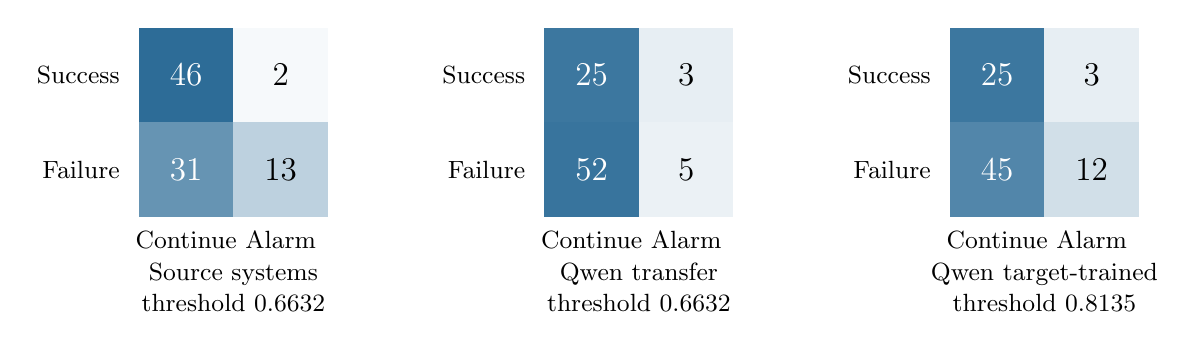
\begin{tikzpicture}[font=\small]
\begin{scope}[xshift=0.0cm]
\fill[preactblue!96!white] (0.0,1.2) rectangle (1.2,2.4);
\node[text=white,font=\large] at (0.6,1.7999999999999998) {46};
\fill[preactblue!4!white] (1.2,1.2) rectangle (2.4,2.4);
\node[text=black,font=\large] at (1.7999999999999998,1.7999999999999998) {2};
\fill[preactblue!70!white] (0.0,0.0) rectangle (1.2,1.2);
\node[text=white,font=\large] at (0.6,0.6) {31};
\fill[preactblue!30!white] (1.2,0.0) rectangle (2.4,1.2);
\node[text=black,font=\large] at (1.7999999999999998,0.6) {13};
\node[anchor=east] at (-.12,1.8) {Success};
\node[anchor=east] at (-.12,.6) {Failure};
\node at (.6,-.3) {Continue};
\node at (1.8,-.3) {Alarm};
\node[align=center,font=\small] at (1.2,-.9) {Source systems\\threshold 0.6632};
\end{scope}
\begin{scope}[xshift=5.15cm]
\fill[preactblue!89!white] (0.0,1.2) rectangle (1.2,2.4);
\node[text=white,font=\large] at (0.6,1.7999999999999998) {25};
\fill[preactblue!11!white] (1.2,1.2) rectangle (2.4,2.4);
\node[text=black,font=\large] at (1.7999999999999998,1.7999999999999998) {3};
\fill[preactblue!91!white] (0.0,0.0) rectangle (1.2,1.2);
\node[text=white,font=\large] at (0.6,0.6) {52};
\fill[preactblue!9!white] (1.2,0.0) rectangle (2.4,1.2);
\node[text=black,font=\large] at (1.7999999999999998,0.6) {5};
\node[anchor=east] at (-.12,1.8) {Success};
\node[anchor=east] at (-.12,.6) {Failure};
\node at (.6,-.3) {Continue};
\node at (1.8,-.3) {Alarm};
\node[align=center,font=\small] at (1.2,-.9) {Qwen transfer\\threshold 0.6632};
\end{scope}
\begin{scope}[xshift=10.3cm]
\fill[preactblue!89!white] (0.0,1.2) rectangle (1.2,2.4);
\node[text=white,font=\large] at (0.6,1.7999999999999998) {25};
\fill[preactblue!11!white] (1.2,1.2) rectangle (2.4,2.4);
\node[text=black,font=\large] at (1.7999999999999998,1.7999999999999998) {3};
\fill[preactblue!79!white] (0.0,0.0) rectangle (1.2,1.2);
\node[text=white,font=\large] at (0.6,0.6) {45};
\fill[preactblue!21!white] (1.2,0.0) rectangle (2.4,1.2);
\node[text=black,font=\large] at (1.7999999999999998,0.6) {12};
\node[anchor=east] at (-.12,1.8) {Success};
\node[anchor=east] at (-.12,.6) {Failure};
\node at (.6,-.3) {Continue};
\node at (1.8,-.3) {Alarm};
\node[align=center,font=\small] at (1.2,-.9) {Qwen target-trained\\threshold 0.8135};
\end{scope}
\end{tikzpicture}
% END INLINE revision_confusion
\caption{Original checkpoint-20 confusion matrices: actual terminal outcome by continue/alarm decision. Counts are exact; shading is row-normalized. The source-validation threshold transfers unchanged to Qwen; target-trained thresholds use target validation. No calibration adaptation is applied in these matrices.}
\label{fig:confusion}
\end{figure*}

\subsection{Partition Sensitivity}
Table~\ref{tab:cv} and Fig.~\ref{fig:sensitivity} show that the single-partition contrast is unstable. At 20 results, repeated grouped transfer AUROC ranges from 0.463 to 0.562, while target-trained AUROC ranges from 0.497 to 0.558. The advantage reverses for one seed; all three paired intervals include zero. Original within-Qwen signal therefore does not establish robust target-training superiority. Full four-checkpoint scores and conditional intervals are retained, including checkpoints where target training performs worse.

\begin{table*}[t]
\centering\footnotesize
\caption{Checkpoint-20 grouped five-fold evaluation. Seeds 20261010--20261012 reuse the same tasks. Fold means are unweighted; parentheses give sample SD, not uncertainty of the mean. All five folds are defined. Paired intervals concern pooled predictions.}
\label{tab:cv}
\begin{tabular}{@{}rrrcrcl@{}}\toprule
Seed & $n$ & Transfer pooled & Transfer fold mean (SD) & Own pooled & Own fold mean (SD) & Pooled $\Delta$ [95\% interval] \\
\midrule
10 & 553 & 0.463 & 0.517 (0.037) & 0.557 & 0.566 (0.061) & 0.094 [-0.001, 0.187] \\
11 & 553 & 0.562 & 0.567 (0.052) & 0.496 & 0.497 (0.116) & -0.065 [-0.151, 0.021] \\
12 & 553 & 0.472 & 0.510 (0.100) & 0.506 & 0.539 (0.085) & 0.034 [-0.054, 0.119] \\
\bottomrule\end{tabular}
\end{table*}

\begin{figure*}[t]
\centering% BEGIN INLINE revision_sensitivity
\begin{minipage}{.49\textwidth}\centering
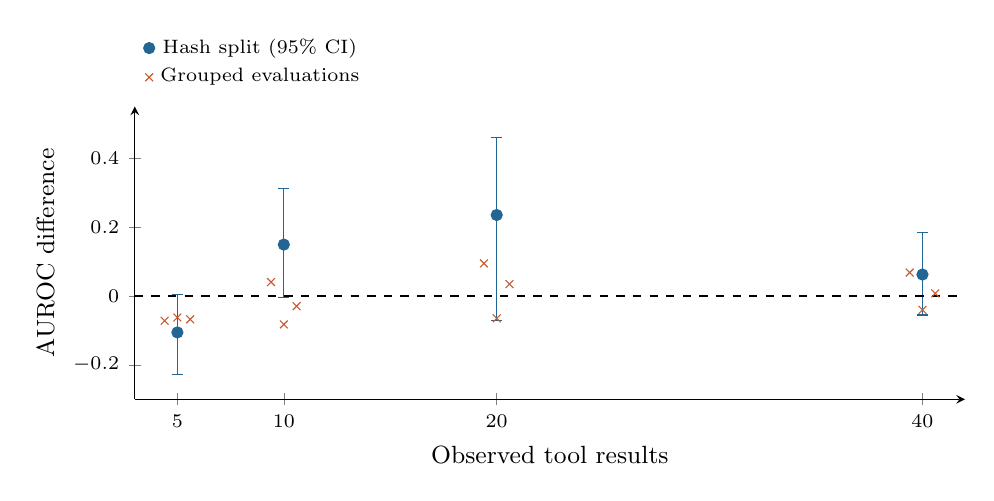
\begin{tikzpicture}
\begin{axis}[font=\small,tick label style={font=\scriptsize},axis lines=left,width=\linewidth,height=5.3cm,xmin=3,xmax=42,ymin=-.30,ymax=.55,xtick={5,10,20,40},xlabel={Observed tool results},ylabel={AUROC difference},legend style={at={(0,1.03)},anchor=south west,draw=none,font=\scriptsize}]
\addplot[only marks,mark=*,preactblue,error bars/.cd,y dir=both,y explicit] table[x=cp,y=difference,y error minus=minus,y error plus=plus] {
cp difference minus plus
5 -0.10588972 0.12254267 0.11069952
10 0.14912281 0.15247668 0.16236348
20 0.23496241 0.30588171 0.22438313
40 0.06211180 0.11749854 0.12152699
};
\addlegendentry{Hash split (95\% CI)}
\addplot[only marks,mark=x,preactorange] coordinates {(4.4,-0.07201979) (5.0,-0.06247163) (5.6,-0.06789638) (9.4,0.04027328) (10.0,-0.08262718) (10.6,-0.02956753) (19.4,0.09445543) (20.0,-0.06504411) (20.6,0.03439306) (39.4,0.06781730) (40.0,-0.04031140) (40.6,0.00761882)};
\addlegendentry{Grouped evaluations}
\addplot[black,dashed,forget plot] coordinates {(3,0)(42,0)};
\end{axis}
\end{tikzpicture}
\end{minipage}\hfill
\begin{minipage}{.49\textwidth}\centering
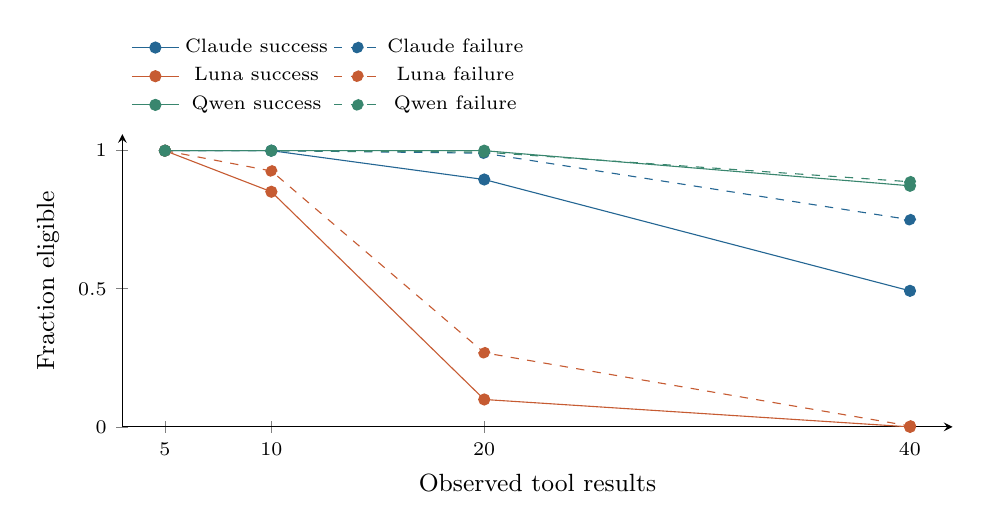
\begin{tikzpicture}
\begin{axis}[font=\small,tick label style={font=\scriptsize},axis lines=left,width=\linewidth,height=5.3cm,xmin=3,xmax=42,ymin=0,ymax=1.06,xtick={5,10,20,40},xlabel={Observed tool results},ylabel={Fraction eligible},legend columns=2,legend style={at={(0,1.03)},anchor=south west,draw=none,font=\scriptsize}]
\addplot[preactblue,solid,mark=*] coordinates {(5,1.00000000) (10,1.00000000) (20,0.89552239) (40,0.49253731)};
\addlegendentry{Claude success}
\addplot[preactblue,dashed,mark=*] coordinates {(5,1.00000000) (10,1.00000000) (20,0.99090909) (40,0.75000000)};
\addlegendentry{Claude failure}
\addplot[preactorange,solid,mark=*] coordinates {(5,1.00000000) (10,0.85123967) (20,0.09917355) (40,0.00000000)};
\addlegendentry{Luna success}
\addplot[preactorange,dashed,mark=*] coordinates {(5,1.00000000) (10,0.92651757) (20,0.26837061) (40,0.00319489)};
\addlegendentry{Luna failure}
\addplot[preactgreen,solid,mark=*] coordinates {(5,1.00000000) (10,1.00000000) (20,1.00000000) (40,0.87283237)};
\addlegendentry{Qwen success}
\addplot[preactgreen,dashed,mark=*] coordinates {(5,1.00000000) (10,1.00000000) (20,0.99476440) (40,0.88743455)};
\addlegendentry{Qwen failure}

\end{axis}
\end{tikzpicture}
\end{minipage}
% END INLINE revision_sensitivity
\caption{Left: original paired task-bootstrap intervals and repeated grouped-CV differences, all checkpoints. Intervals condition on fitted models. Right: outcome-stratified prefix eligibility over all runs; solid denotes success and dashed failure. The moving risk sets are strongly system-dependent.}
\label{fig:sensitivity}
\end{figure*}

At checkpoint 20, within-fold transfer means are 0.517--0.567 and target-trained means 0.497--0.566 (Table~\ref{tab:cv}); the advantage again changes sign. These comparisons avoid ranking examples across different fold models. The archive reports every fold AUROC and its sample size at all four checkpoints.

\subsection{Checkpoint Eligibility and Common Cohorts}
At 20 results, 300/335 successful and 218/220 failed Claude runs are eligible, versus only 24/242 successful and 84/313 failed Luna runs. Qwen retains 173/173 successes and 380/382 failures. Thus the pooled source cohort at later checkpoints becomes heavily reweighted toward Claude and long Luna failures. Differences in counts, duration and task composition can contribute to apparent transfer effects.

On the common all-system task/run cohort at 20 results, only 16 target-test runs remain: transfer/own AUROC is 0.564/0.691, versus 0.456/0.691 on the original 85 Qwen runs. No all-system common test runs remain at 40 results. Restricting instead to the fixed 74 Qwen runs reaching 40 results gives checkpoint-20 AUROC 0.480/0.665. These conditional results demonstrate sensitivity without eliminating selection bias, isolating harness effects, or supporting a deployable future-duration rule.

\subsection{Target Adaptation and Feature Drift}
At 20 results, prior adjustment improves Brier from 0.300 to 0.245 and target-validation logistic recalibration to 0.229; neither changes AUROC 0.456 because both maps are increasing. A constant target-validation failure prior has Brier 0.223, better than either adapted score; adaptation does not establish predictive benefit beyond this control. The ECDF baseline yields AUROC 0.446 and Brier 0.463. Table~\ref{tab:adapt} retains AP. Adaptation is not consistently beneficial: checkpoint-40 logistic recalibration slope is negative and AUROC falls from 0.551 to 0.449, with Brier rising from 0.229 to 0.265. Target validation cannot guarantee test calibration.

\begin{table}[t]
\centering\footnotesize
\caption{Checkpoint-20 Qwen test metrics. Target adaptation fits only the 16 validation tasks; no test-label fitting.}
\label{tab:adapt}
\begin{tabular}{@{}lrrr@{}}\toprule Method & AUROC & AP & Brier \\
\midrule
Unchanged source & .456 & .647 & .300 \\
Target-validation prior & .500 & .671 & .223 \\
Prior correction & .456 & .647 & .245 \\
Logistic recalibration & .456 & .647 & .229 \\
ECDF normalization & .446 & .672 & .463 \\
Target-trained & .691 & .795 & .200 \\
\bottomrule\end{tabular}
\end{table}

\begin{figure*}[t]
\centering% BEGIN INLINE revision_shift
\begin{minipage}{.49\textwidth}\centering
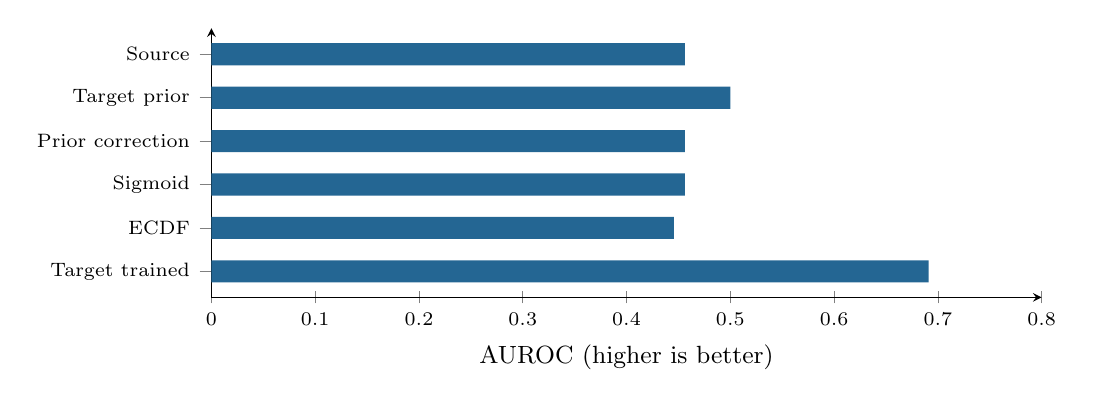
\begin{tikzpicture}
\begin{axis}[font=\small,tick label style={font=\scriptsize},axis lines=left,width=\linewidth,height=5.0cm,xbar,bar width=8pt,xmin=0,xmax=0.8,ymin=.4,ymax=6.6,ytick={1,2,3,4,5,6},yticklabels={Target trained,ECDF,Sigmoid,Prior correction,Target prior,Source},xlabel={AUROC (higher is better)}]
\addplot[fill=preactblue,draw=none] coordinates {(0.4561,6) (0.5000,5) (0.4561,4) (0.4561,3) (0.4455,2) (0.6911,1)};
\end{axis}
\end{tikzpicture}
\end{minipage}\hfill
\begin{minipage}{.49\textwidth}\centering
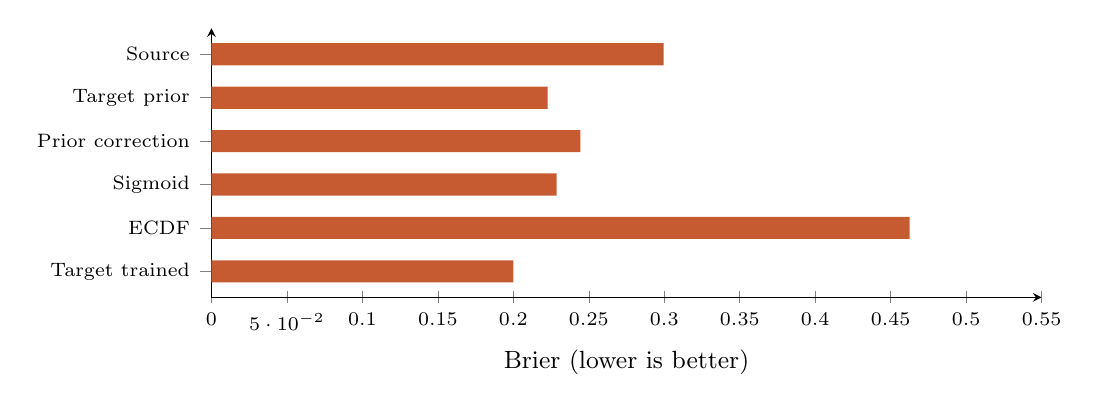
\begin{tikzpicture}
\begin{axis}[font=\small,tick label style={font=\scriptsize},axis lines=left,width=\linewidth,height=5.0cm,xbar,bar width=8pt,xmin=0,xmax=0.55,ymin=.4,ymax=6.6,ytick={1,2,3,4,5,6},yticklabels={Target trained,ECDF,Sigmoid,Prior correction,Target prior,Source},xlabel={Brier (lower is better)}]
\addplot[fill=preactorange,draw=none] coordinates {(0.2996,6) (0.2227,5) (0.2445,4) (0.2287,3) (0.4626,2) (0.2001,1)};
\end{axis}
\end{tikzpicture}
\end{minipage}
% END INLINE revision_shift
\caption{Checkpoint-20 AUROC and Brier shown separately with horizontal method labels. Higher AUROC and lower Brier are preferred; results are retained in Table~\ref{tab:adapt}. Sigmoid denotes target-validation logistic recalibration. Feature-shift graphics and all diagnostics are supplementary.}
\label{fig:shift}
\end{figure*}

Validation feature distributions differ substantially; all 20 standardized differences and KS distances are supplied. They establish covariate differences between observed cohorts, not model-weight causality or stable conditional-label relations. Rank normalization and prevalence correction test limited alternatives; richer semantic monitors, more systems and independent model/scaffold factorial comparisons remain unperformed.

\section{Reproducibility and Limitations}
The reproducibility package includes task IDs/splits, selected source-index records, compressed/decompressed hashes, dependency versions, scripts, aggregate JSONs and complete reports. Downloads use the verified Hub commit; raw traces remain at the source and are excluded from redistribution. A clean pinned Python 3.13.5 environment (NumPy 2.2.6, SciPy 1.15.3, scikit-learn 1.6.1) reproduced the four original analyses exactly and all revision numerical fields within $10^{-8}$. This verifies environment portability on the same data/code, not independent-data replication. Regeneration requires no language-model API or GPU. Materials are available at \url{https://github.com/f20230006-sketch/preact-reproducibility}. No conference submission has been made. Evidence-map judgments remain single-reviewer extraction.

A previous one-thread CPU audit (Windows 11, Python 3.13.5, scikit-learn 1.6.1) extracted 5,271 prefix rows in 2.85 s and fit two checkpoint-20 candidates in 0.035 s; median warmed batch inference over 92 rows was 0.763 ms. These timings exclude downloads, agent execution and orchestration, establishing neither energy savings nor online latency. The prior environment's NumPy metadata discrepancy and non-fatal optimizer warning are documented; the clean rerun eliminates these issues.

This study uses one dataset, only three jointly changing model/scaffold systems, terminal labels, and reused tasks across sensitivity seeds. Checkpoint selection and new analyses are exploratory. Outcome-stratified eligibility and common cohorts do not identify missing-prefix population performance. Conditional bootstrap intervals omit full training uncertainty, and pooled cross-fitted scores can differ in scale. A monitor that performs near chance after transfer should not control unsupported systems automatically. Source traces may contain sensitive repository content; aggregates avoid redistributing raw content. Subgroup fairness and intervention safety are unmeasured.

Future work should independently vary model and scaffold, evaluate another dataset, and compare structural with semantic/event monitors under shared tasks and budgets. Establishing prevention requires observable-error-time annotations and randomized continuation/verification/restart branches with matched total budgets and a resampling control~\cite{sentinel,dover}. Measure both recovery and disruption, not classifier accuracy alone. The complete proposed intervention protocol is supplementary and is not an implemented system.

\section{Conclusion}
The original task partition suggests a cross-system reliability problem, but paired uncertainty and repeated grouped evaluation do not establish a stable target-training advantage. Checkpoint eligibility changes the compared populations. Target-validation adaptation can improve probability error without recovering ranking or beating a constant target prior, and can degrade later performance. The evaluation protocol exposes how a promising single-split result becomes inconclusive under stronger paired, task-grouped, eligibility and calibration analyses. This reliability-audit contribution supports reporting those checks alongside headline metrics. They demonstrate neither prevention nor a model-only transfer effect.

\IEEEtriggeratref{9}
\begin{thebibliography}{99}
\bibitem{react} S. Yao \emph{et al.}, ``ReAct: Synergizing reasoning and acting in language models,'' in \emph{ICLR}, 2023.
\bibitem{reflexion} N. Shinn \emph{et al.}, ``Reflexion: Language agents with verbal reinforcement learning,'' in \emph{NeurIPS}, 2023.
\bibitem{sweprm} S. Gandhi \emph{et al.}, ``When agents go astray: Course-correcting SWE agents with PRMs,'' arXiv:2509.02360, 2025.
\bibitem{selfhealing} C. Jeong and Y. Shin, ``A self-healing framework for reliable LLM-based autonomous agents,'' arXiv:2605.06737, 2026.
\bibitem{prefixguard} X. Huang \emph{et al.}, ``PrefixGuard: Online failure warning and trace-grounded diagnosis for LLM agents,'' arXiv:2605.06455, 2026.
\bibitem{sparse} A. Baidya \emph{et al.}, ``When evidence is sparse: Weakly supervised early failure alerting in dialogs and LLM-agent trajectories,'' arXiv:2606.05414, 2026.
\bibitem{failfast} C. Wang \emph{et al.}, ``Fail-Fast, Restart-Smart: Early failure prediction and restart for SWE agentic tasks,'' arXiv:2608.03222, 2026.
\bibitem{interventionparadox} R. Vasudev \emph{et al.}, ``Accurate failure prediction in agents does not imply effective failure prevention,'' arXiv:2602.03338, 2026.
\bibitem{agentforesight} B. Zhang \emph{et al.}, ``AgentForesight: Online auditing for early failure prediction in multi-agent systems,'' arXiv:2605.08715, 2026.
\bibitem{graphcopilot} X. Zheng \emph{et al.}, ``Leveraging trajectory graphs for pre-execution error diagnosis in agentic LLM systems,'' arXiv:2607.27443, 2026.
\bibitem{earlyeval} Y. Shi \emph{et al.}, ``EarlyEval: Cheaper agent evaluation via early outcome prediction,'' arXiv:2609.02783, 2026.
\bibitem{agentstop} D. Pham \emph{et al.}, ``AgentStop: Terminating local AI agents early to save energy in consumer devices,'' arXiv:2605.15206, 2026.
\bibitem{atropos} N. Kim and S. Yoo, ``Atropos: Improving cost-benefit trade-off of LLM-based agents under self-consistency with early termination and model hotswap,'' arXiv:2604.15075, 2026.
\bibitem{calibrationaudit} Y. Cao, ``Testing-Driven Reliability Audit of Trajectory-Based Early Outcome Prediction for LLM Agents: Target-Specific Calibration Transfer Persists Within a Single Benchmark,'' arXiv:2609.25647, 2026.
\bibitem{agentrewardbench} X. H. L\`u \emph{et al.}, ``AgentRewardBench: Evaluating automatic evaluations of web agent trajectories,'' arXiv:2504.08942, 2025.
\bibitem{rebench} ibragim-bad, ``SWE-Rebench July 2026 trajectories,'' Hugging Face dataset, 2026. [Online]. Available: \url{https://huggingface.co/datasets/ibragim-bad/swe_rebench_07_2026_trajectories}
\bibitem{sentinel} S. Dubey, ``Real-Time Detection and Repair of LLM Agent Failures,'' arXiv:2608.02464, 2026.
\bibitem{probguard} H. Wang, C. M. Poskitt, J. Wei, and J. Sun, ``ProbGuard: Proactive Runtime Monitoring for LLM Agent Safety via Probabilistic Prediction,'' arXiv:2508.00500, 2025.
\bibitem{agentspec} H. Wang, C. M. Poskitt, and J. Sun, ``AgentSpec: Customizable Runtime Enforcement for Safe and Reliable LLM Agents,'' arXiv:2503.18666, 2025.
\bibitem{promas} X. Zhao \emph{et al.}, ``ProMAS: Proactive Error Forecasting for Multi-Agent Systems Using Markov Transition Dynamics,'' arXiv:2603.20260, 2026.
\bibitem{dover} M. Ma \emph{et al.}, ``DoVer: Intervention-Driven Auto Debugging for LLM Multi-Agent Systems,'' arXiv:2512.06749, 2025.
\bibitem{a2p} A. West \emph{et al.}, ``Abduct, Act, Predict: Scaffolding Causal Inference for Automated Failure Attribution in Multi-Agent Systems,'' arXiv:2509.10401, 2025.
\bibitem{agentlens} P. Sahoo \emph{et al.}, ``AgentLens: Revealing The Lucky Pass Problem in SWE-Agent Evaluation,'' arXiv:2605.12925, 2026.
\bibitem{failureprocess} X. Zhao \emph{et al.}, ``Failure as a Process: An Anatomy of CLI Coding Agent Trajectories,'' arXiv:2607.09510, 2026.
\end{thebibliography}
\end{document}
